\begin{frame}
	\frametitle{Adaptive Sampling: Theory}
	 \begin{columns}[onlytextwidth,T]
      \column{\dimexpr\linewidth-6cm-5mm}
        
        How to take advantage of surrogate information content \textit{during training} to reduce sample quantity? \newline
        
		We developed \alert{a new technique:}
        \vspace{-1em}
        \begin{enumerate}
        \item Construct surrogate quality distribution by nearest- neighbour interpolation.
        \item Draw candidate samples by quality using MCMC.
        \item Include samples with greatest separation from neighbours.
        \item Repeat!
        \end{enumerate}
      \column{6cm}
      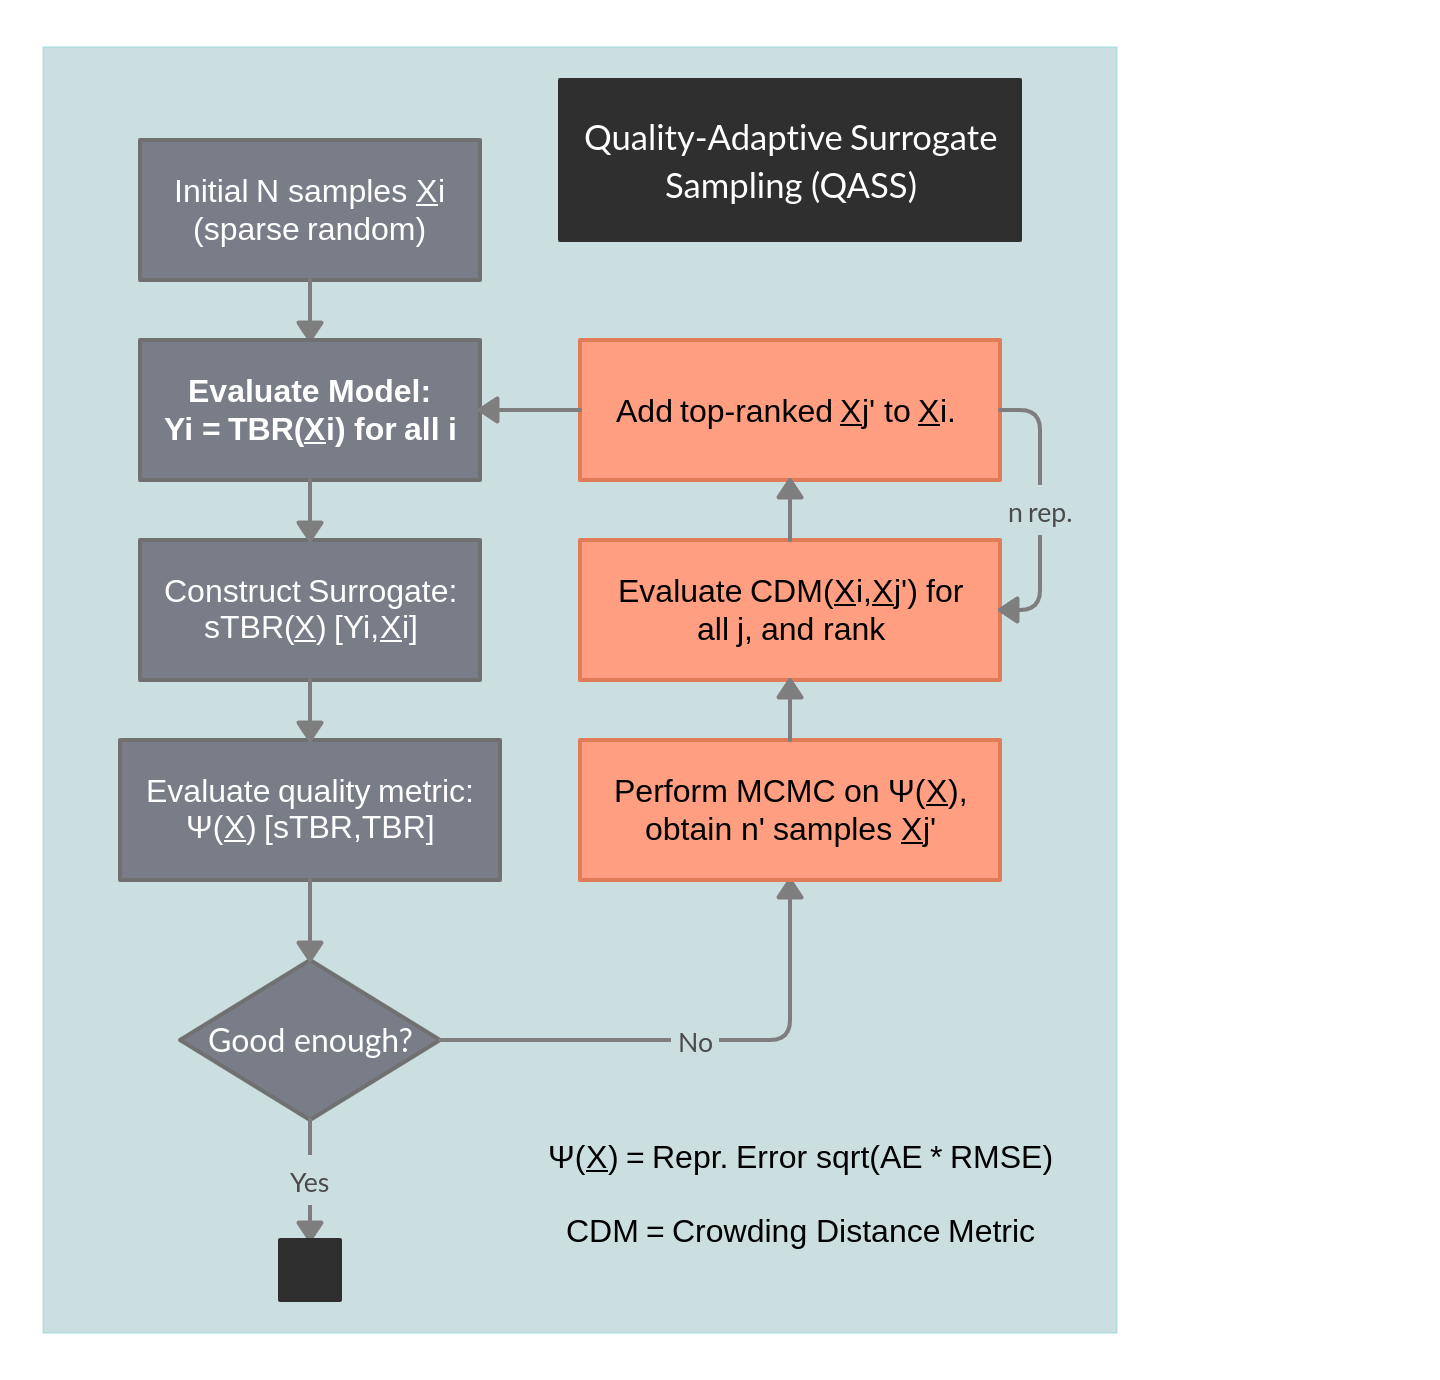
\includegraphics[width=8cm]{qassplan}

    \end{columns}
\end{frame}

\begin{frame}
	\frametitle{Application on Toy Theory}
	Toy functional TBR theory with wavenumber $n$, and qualitatively comparable ANN performance to Paramak:
	\begin{align*}
		\text{TBR}_\text{toy} = \frac{1}{|C|}\sum_{i \in C} \left[1 + \sin(2\pi n (x_i - 1/2)) \right]
	\end{align*}

	\vspace{-1em}
	{\footnotesize
		\hfill(where $C$~enumerates all continuous variables)
	}

	\vspace{1em}

	\begin{columns}[T]
		\column{0.5\paperwidth}
		\vspace{-0.5em}
		Evaluation set:
		\begin{itemize}
		    \item Adaptive samples
		    \item Generated during runtime
		\end{itemize}
		\vspace{0.5em}
		Validation set:
		\begin{itemize}
		    \item Uniform random samples
		    \item Generated independently
		\end{itemize}
		\vspace{15pt}

		Placebo comparison -- incremental uniform-random samples, no MCMC.


		\column{0.4\paperwidth}
		\hspace{-20pt}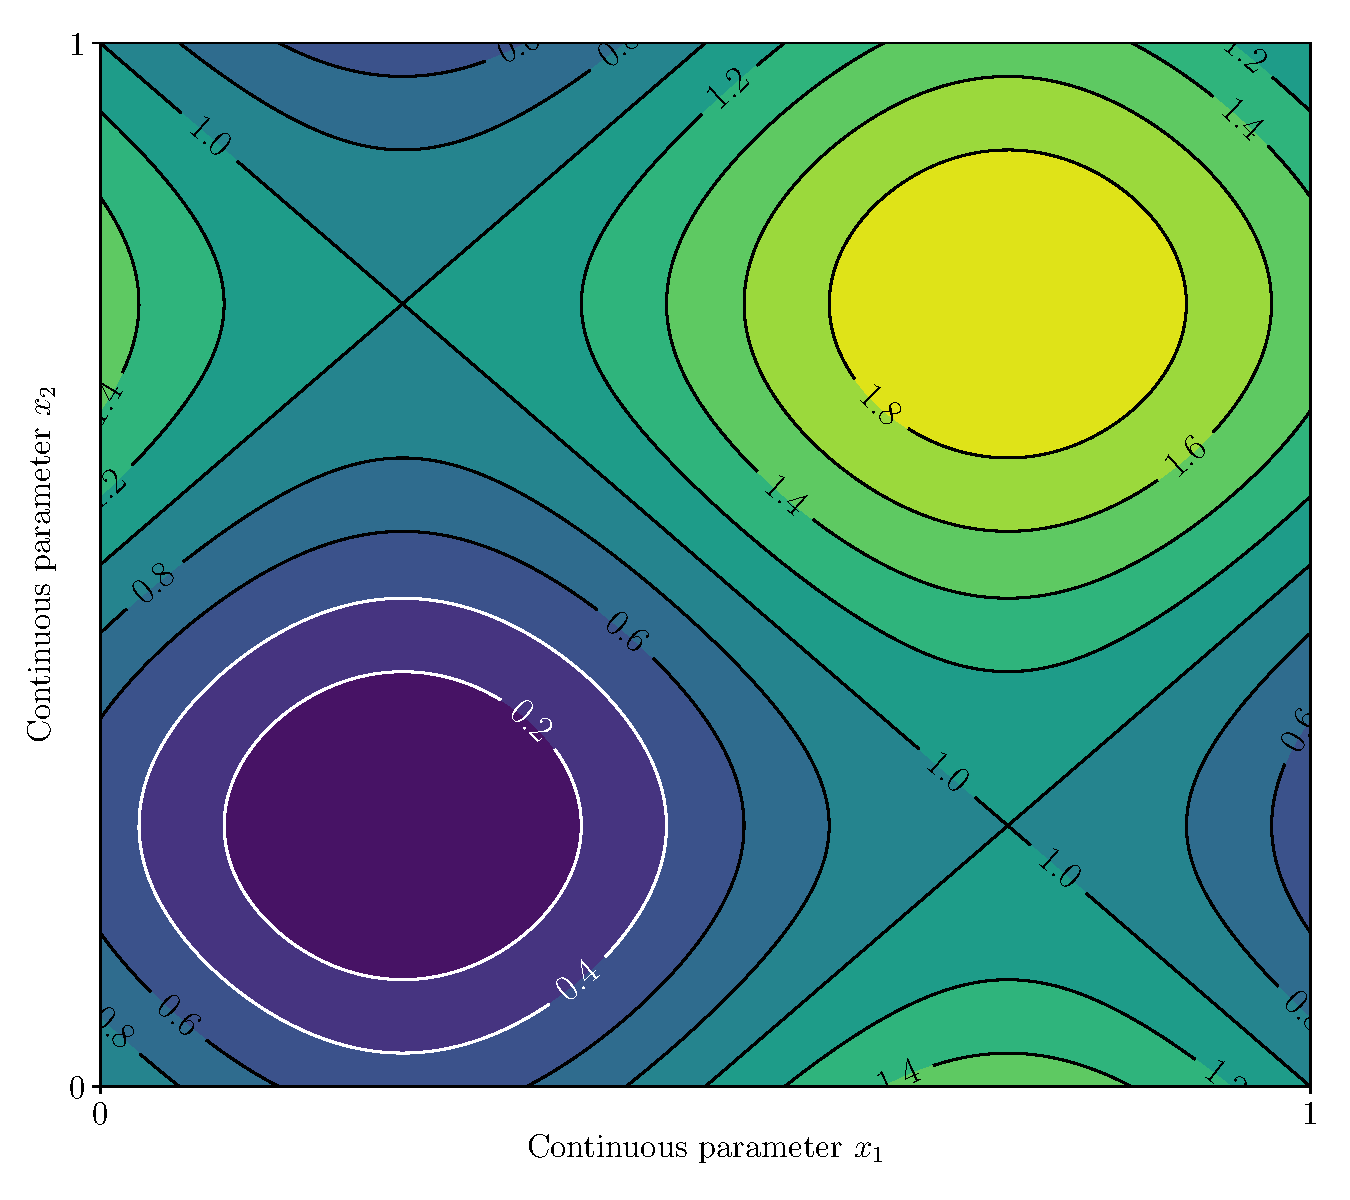
\includegraphics[width=0.45\paperwidth]{sintoy}

	\end{columns}
\end{frame}

\begin{frame}
    \frametitle{Adaptive Sampling: Results}
    \vspace{-20pt}
    \begin{center}
    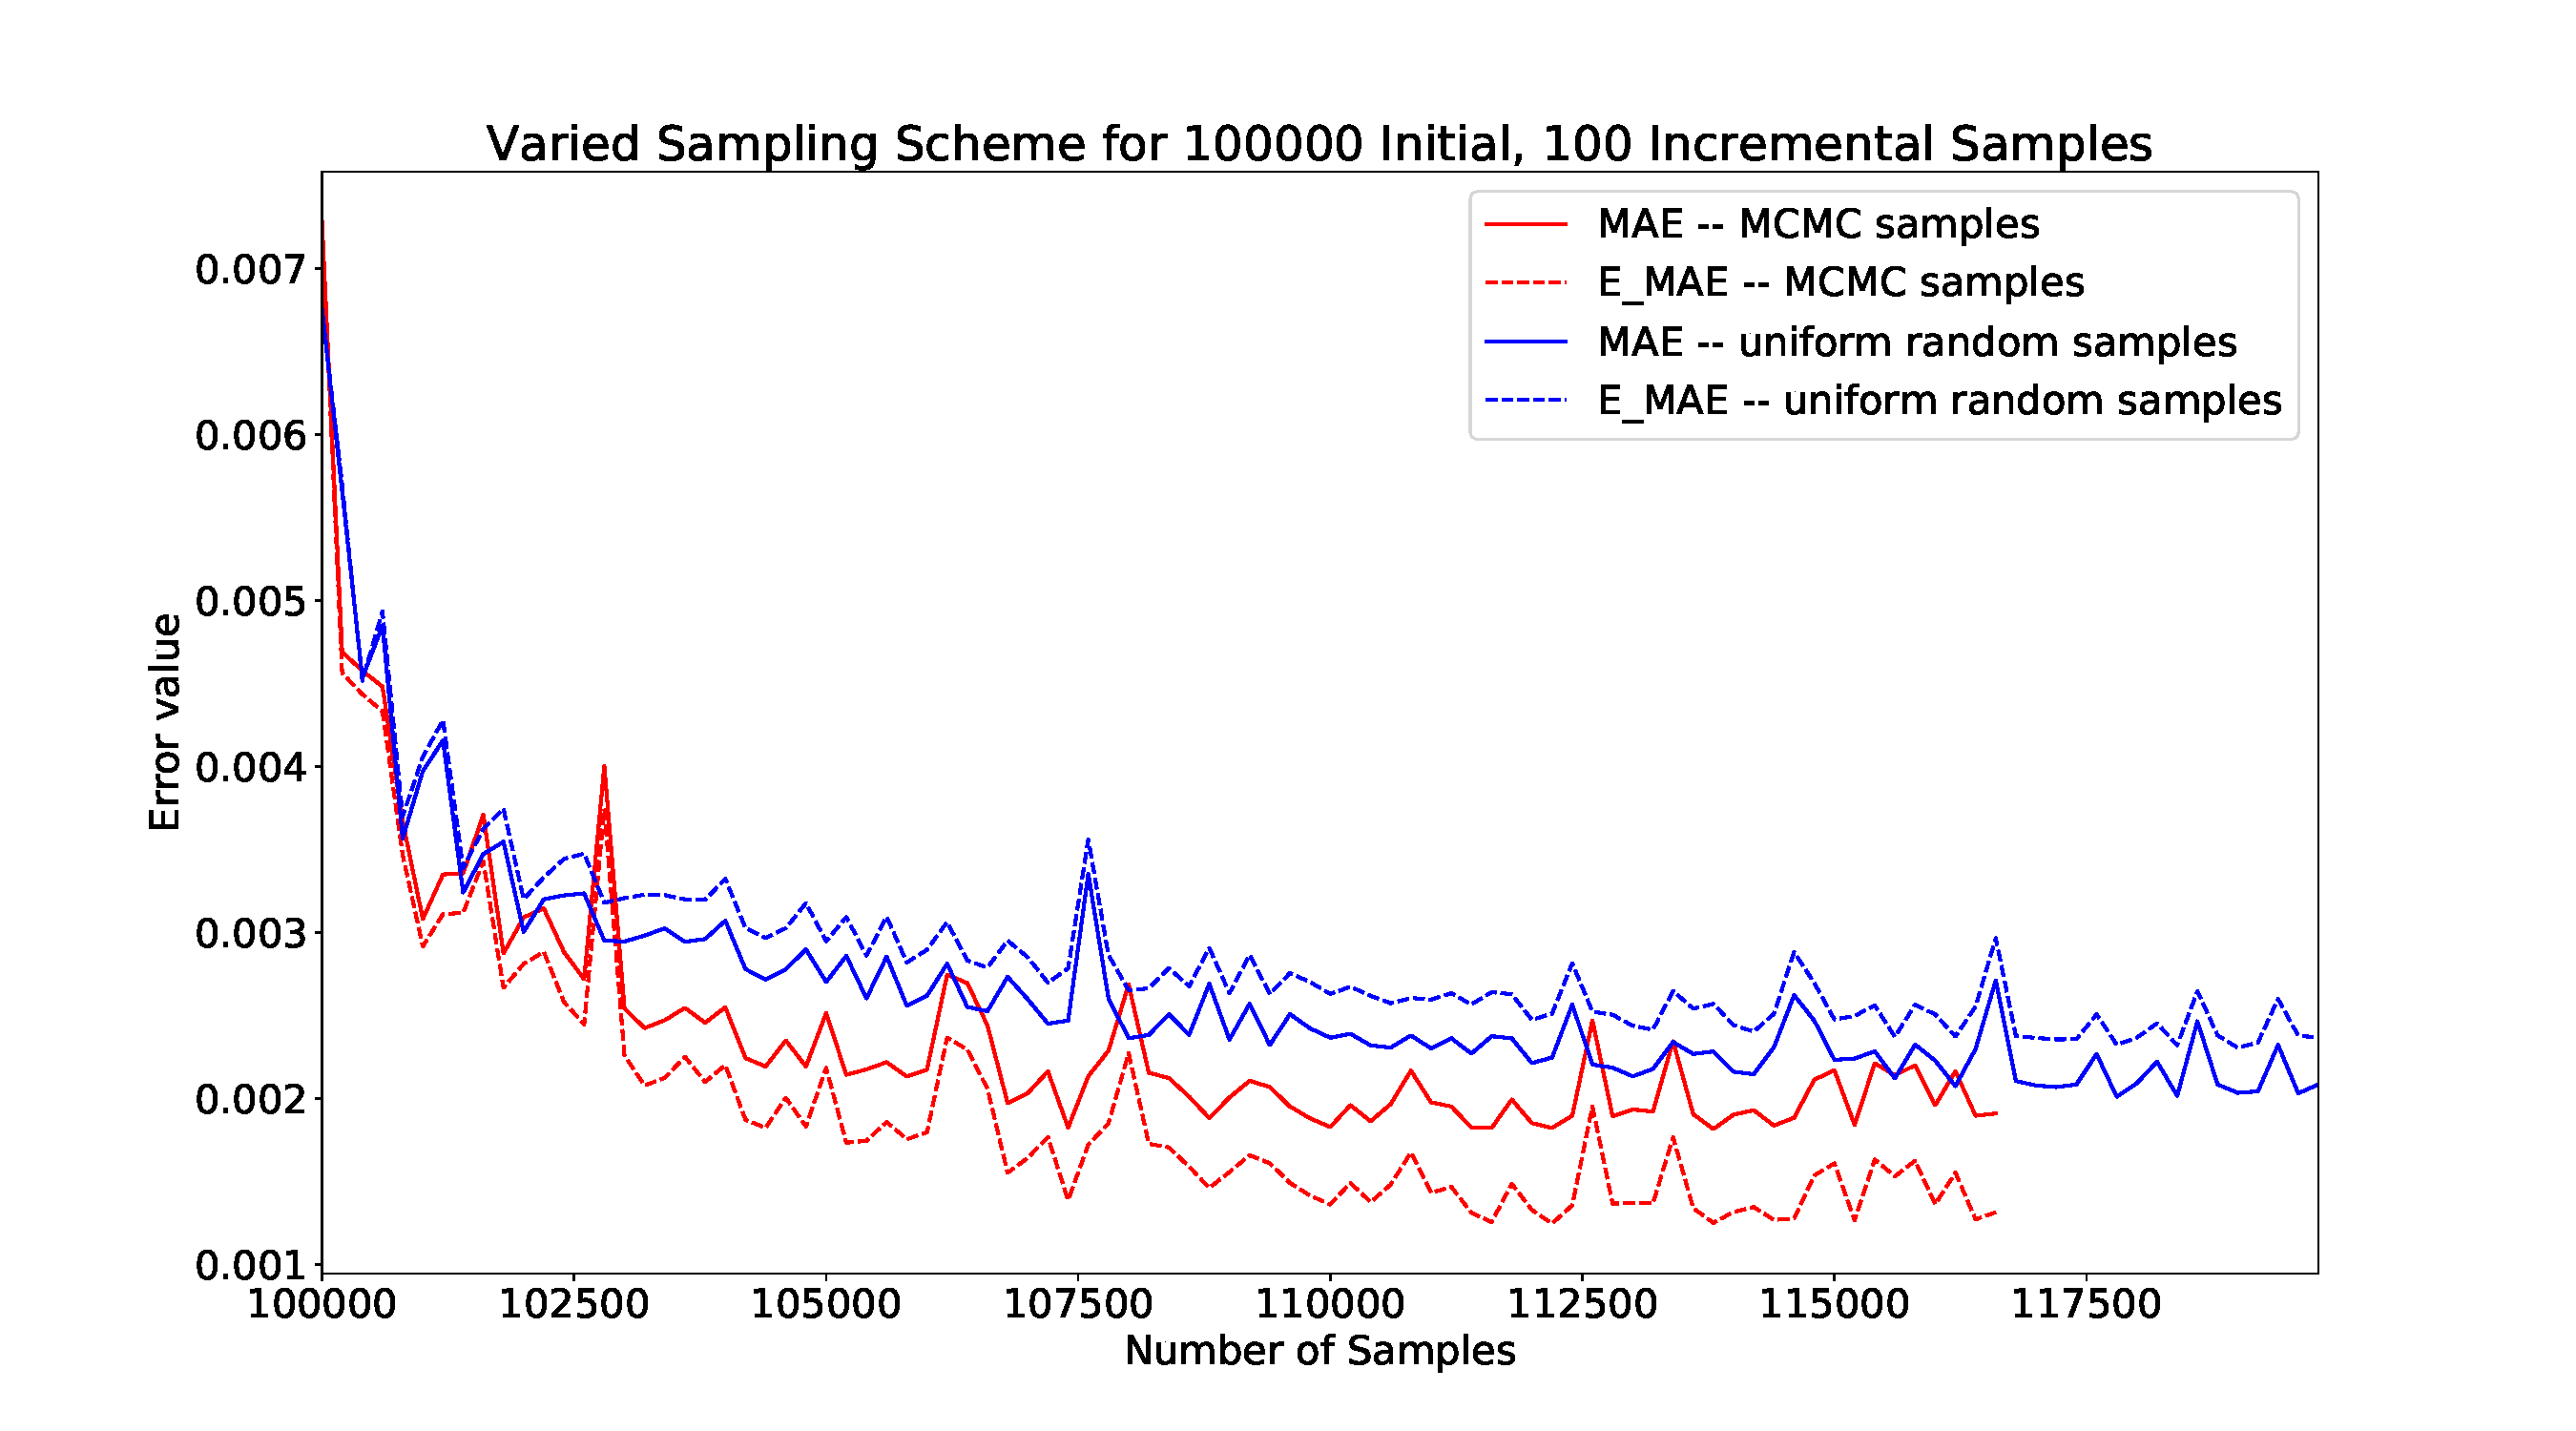
\includegraphics[width=12cm]{qassresult}
    \end{center}
    
	\alert{$60\%$ decrease} in MAE for validation set (dashed) \newline
	Equivalently, \alert{$6\%$ decrease} in samples needed for same accuracy

\end{frame}


\begin{frame}
    \frametitle{Adaptive Sampling: Results}
    \vspace{-20pt}
    \begin{center}
    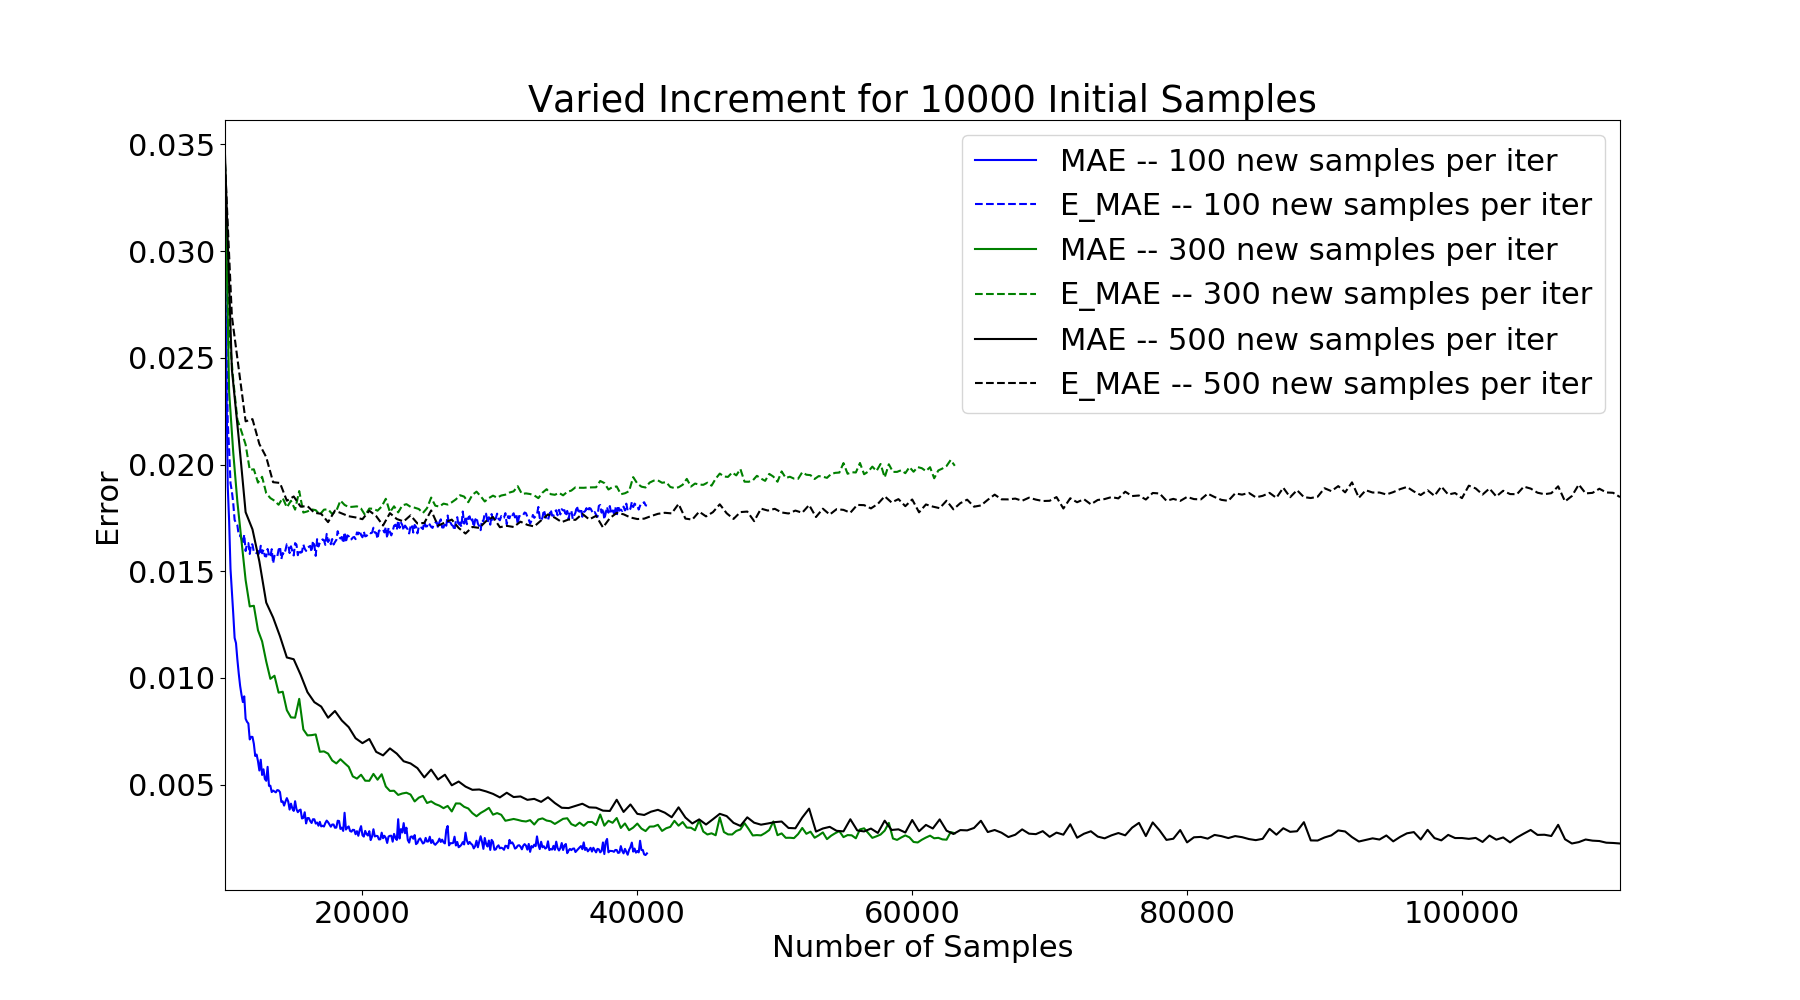
\includegraphics[width=12cm]{qassincr}
    \end{center}
    
    Fewer incremented samples can lead to better accuracy! \newline
    But depends on initial samples, specific model -- further study needed.

\end{frame}
